\documentclass{standalone}
\usepackage{tikz}
\usepackage{hsbcommon}

\begin{document}
    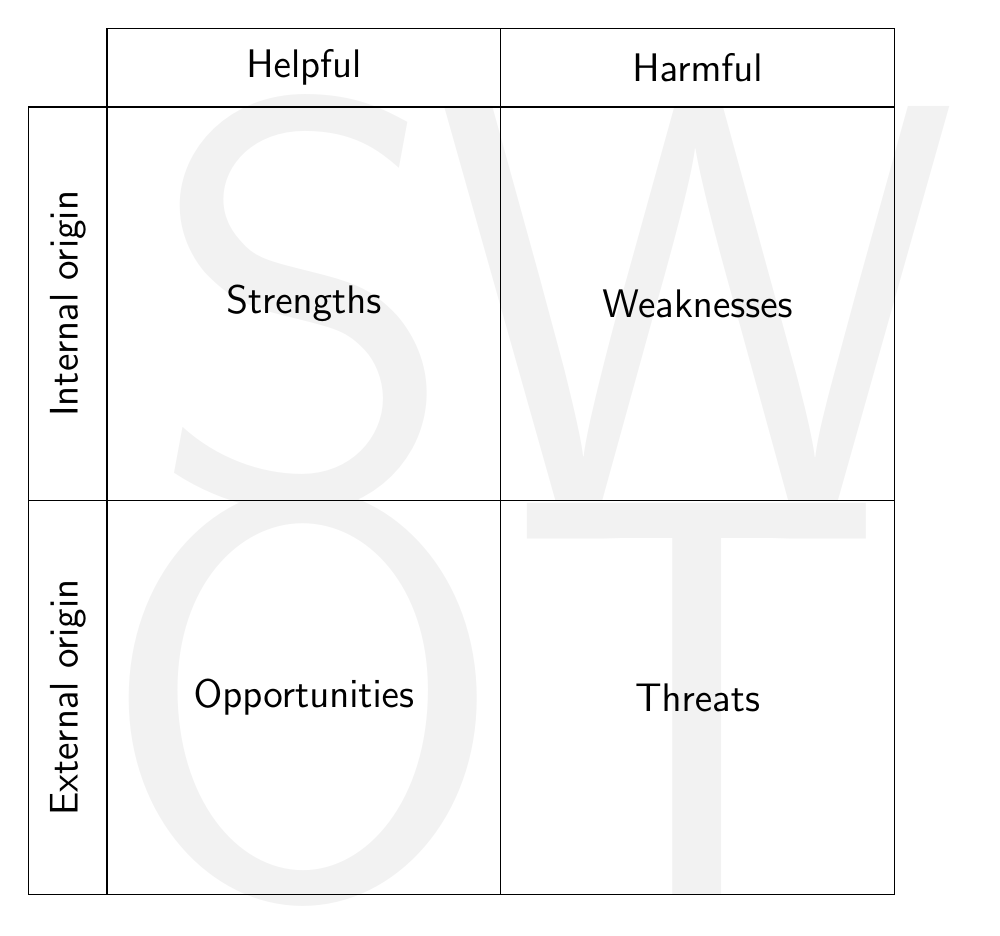
\begin{tikzpicture}[every node/.style={font=\sffamily}]\Large

            \tikzset{every node/.style={
                color=gray!10,
                font=\sffamily
            }}
            \node (s) at (0,5) {
                \resizebox{!}{5cm}{S}
                };

            \node (w) at (5,5) {
                \resizebox{!}{5cm}{W}
                };

            \node (o) at (0,0) {
                \resizebox{!}{5cm}{O}
                };

            \node (t) at (5,0) {
                \resizebox{!}{5cm}{T}
                };

            
            
            \tikzset{
            every node/.style={
                draw,
                text width=15ex,
                minimum height=5cm,
                minimum width=5cm,
                text centered,
                font=\sffamily
            }
        }
        
           \node at (s) {Strengths};
           \node at (w) {Weaknesses};
           \node at (o) {Opportunities};
           \node at (t) {Threats};

            \tikzset{
            every node/.style={
                draw,
                text width=15ex,
                minimum height=1cm,
                minimum width=5cm,
                text centered,
                font=\sffamily
            }
        }

        \node at (s |-,8) {Helpful};
        \node at (w |-,8) {Harmful};
        \node[rotate=90] at (-3, |- s) {Internal origin};
        \node[rotate=90] at (-3, |- o) {External origin};
        
    \end{tikzpicture}
\end{document}